\title{Answers to Problem Set 1}
\author{
				Lauren Hinkle (lhinkle)\\
        Pedro d'Aquino  (pdaquino)\\
				Robert Goeddel (rgoeddel)\\
        Yash Chitalia (yashc)}
\date{\today}

\documentclass[12pt]{article}
\usepackage{graphicx}
\usepackage{amsmath}

\begin{document}
\maketitle

\section{Task 1: Linear Algebra Review}

\paragraph{A}
Let $A$ be a matrix with the property $AA^T = I$ where $A$ is an $m\times n$ matrix.  Then it must be that $r_i$ is orthogonal to $r_j$ for all rows $r_i, r_j \in A$.  Additionally, $m \leq n$, this is explained in 1C.

\paragraph{B}
\begin{equation*}
A = \left[ \begin{array}{ccc} 1 & 0 & 0 \\ 0 & 1 & 0 \end{array} \right]
\end{equation*}

Proof: \\
\begin{align*}
AA^T:\hspace{10 mm}
\left[ \begin{array}{ccc} 1 & 0 & 0 \\ 0 & 1 & 0 \end{array} \right]
\left[ \begin{array}{cc} 1 & 0  \\ 0 & 1 \\ 0 & 0 \end{array} \right]
&=\left[ \begin{array}{cc} 1 & 0  \\ 0 & 1 \end{array} \right] \\
A^TA:\hspace{10 mm}
\left[ \begin{array}{cc} 1 & 0  \\ 0 & 1 \\ 0 & 0 \end{array} \right]
\left[ \begin{array}{ccc} 1 & 0 & 0 \\ 0 & 1 & 0 \end{array} \right]
&=\left[ \begin{array}{ccc} 1 & 0 & 0  \\ 0 & 1 & 0 \\ 0 & 0 & 0 \end{array} \right]
\end{align*}


\paragraph{C}
Let $A$ be an $m \times n$ matrix such that $AA^T=I$. We can decompose $AA^T$ using SVD:

\[
AA^T = USV^T\left(USV^T\right)^T = USV^TVS^TU^T\]

Because $V$ is orthonormal, $VV^T=I$ and:

\[
AA^T = USS^TU^T
\]

For $AA^T=I$, $SS^T=I$. This follows from the fact that $U$ is orthonormal.

If we expand $A^TA$ using SVD, we reach:

\[
A^TA = VS^TSV^T
\]

For $A^TA$ to be $I$, then $S^TS=I$. But we know that $SS^T$ is also $I$, so these conditions must hold simultaneously for $A^TA=I$.

Recall that $S$ is diagonal and has the same dimensions as $A$. If it is also square, then those conditions can hold simultaneously because $SS^T=S^TS$. However, if $S$ is rectangular, at least one row or column will have nothing but zeroes. In this case, there is only one direction in which multiplying $S$ and $S^T$ yields $I$; in the other direction the result will be a square matrix with at least one row and column equal to zero.

\paragraph{D}
Classes of matrices for which $AA^T = I$ and $A^TA=I$ will hold are square matrices, orthogonal (by definition of an orthogonal matrix), and symmetric.

\section{Task 2: Multiavariate Gaussians}

\paragraph{A}
Let $N$ be the number of samples, $K$ be the number of random variables in $\mathbf{x}$ and $\mathbf{\mu}$ be the sample mean vector. The $i$-th sample of the random variable $\mathbf{x}_k$ is denoted by $\mathbf{x}_{ik}$ Then each element of $\mathbf{\mu}$ is going to be of the form:

\begin{equation}
\mu_k = \frac{1}{N}\displaystyle\sum_{i=1}^{N}{x_{ik}}, k=1,2,...,K
\end{equation}

And every element $\sigma_{jk}$ of the $K \times K$ covariance matrix $\Sigma$ will be given by:

\begin{equation}
\sigma_{jk}=\frac{1}{N-1}\displaystyle\sum_{i=1}^{N}{(x_{ij}-\mu_j)(x_{ik}-\mu_{k})}
\end{equation}

\paragraph{B}

We first prove that for any $m \times n$ matrix $A$, $AA^T$ is SPD. Let $x$ be any column vector of dimensions $m\times1$ and let

\[
\underbrace{x^T}_{1\times m}\underbrace{A}_{m\times n}=\underbrace{t}_{1\times n}
\]

Then:

\[
x^TAA^Tx = \underbrace{t}_{1\times n}\underbrace{t^T}_{n \times 1} = \underbrace{s}_{1\times 1}
\]

Additionaly, $s\geq 0$:

\[s = \displaystyle\sum_{i=1}^n{t_i^2}\]

Therefore, $AA^T$ is SPD. We can extend this to prove that any covariance matrix is also SPD. Again, let $x$ be any column vector of dimensions $m\times1$. We need to prove that $x^T\Sigma x \geq 0$.

\[
x^T\Sigma x=x^TE\left[\left(X-E[X]\right)\left(X-E[X]\right)^T\right]x
\]

Let $A=X-E[X]$. Then we rewrite the equation as:

\[
x^T\Sigma x=x^TE\left[AA^T\right]x = E\left[x^TAA^Tx\right]
\]

But we have already proved that $x^TAA^Tx$ is a scalar $s$, $s \geq 0$:

\[
x^T\Sigma x  =E\left[s\right] \geq 0
\]

\paragraph{C}
Let $Z$ be a multivariate distribution comprised of independent standard normal univariate distributions. Then the mean $\mu_Z = 0$ and the covariance $\Sigma_Z=I$, the identity matrix. If we apply a linear transformation of the form $AZ + b$, we will have a multivariate normal distribution of the form:

\[
\mathcal{N}\left(A\mu_Z + b, A\Sigma_Z A^T\right) = \mathcal{N}\left(A0 + b, BIB^T\right) = \mathcal{N}\left(b, AA^T\right)
\]

Therefore, we can draw from $\mathcal{N}\left(\mu,P\right)$ by making $b=\mu$ and $AA^T=P$ (using, for instance, Cholesky decomposition).

\paragraph{D}
Let there be a two-dimensional distribution with given covariance $\Sigma$ such that there is a $\chi^2$ error of $c$ for some point $p$ where $p = \mu +
\left[ {\begin{smallmatrix}
\alpha cos(\theta)  \\
\alpha sin(\theta)  \\
 \end{smallmatrix} } \right]$
with a given value of $\theta$ and unknown $\alpha$.

By definition, $\chi^2 = \mathbf{w}^T \Sigma^{-1} \mathbf{w}$ where $\mathbf{w} = \mathbf{p}-\mathbf{\mu}$.  Then
\begin{align*}
\mathbf{w} &= \mu +
	\left[ {\begin{smallmatrix}
	\alpha cos(\theta)  \\
	\alpha sin(\theta)  \\
 	\end{smallmatrix} } \right]
	- \mu \\
 &= \alpha \left[ {\begin{smallmatrix}
	cos(\theta)  \\
	sin(\theta)  \\
	 \end{smallmatrix} } \right]
\end{align*}
And therefore the unknown $\alpha$ can be calculated.
\begin{align*}
\chi^2 = c &=  \mathbf{w}^T \Sigma^{-1} \mathbf{w} \\
&=  \alpha \left[ {\begin{smallmatrix}
	cos(\theta)  sin(\theta)  \\
	 \end{smallmatrix} } \right]
 	\Sigma
 	\alpha \left[ {\begin{smallmatrix}
	cos(\theta)  \\
	sin(\theta)  \\
	 \end{smallmatrix} } \right] \\
&= \alpha^2 \left[ {\begin{smallmatrix}
	cos(\theta)  sin(\theta)  \\
	 \end{smallmatrix} } \right]
 	\Sigma
 	\left[ {\begin{smallmatrix}
	cos(\theta)  \\
	sin(\theta)  \\
	 \end{smallmatrix} } \right] \\
\alpha^2 &= \frac{c}{\left[ {\begin{smallmatrix}
	cos(\theta)  sin(\theta)  \\
	 \end{smallmatrix} } \right]
 	\Sigma
 	\left[ {\begin{smallmatrix}
	cos(\theta)  \\
	sin(\theta)  \\
	 \end{smallmatrix} } \right]} \\
\alpha &=\pm\sqrt{ c \left( \left[ {\begin{smallmatrix}
	cos(\theta)  sin(\theta)  \\
	 \end{smallmatrix} } \right]
 	\Sigma
 	\left[ {\begin{smallmatrix}
	cos(\theta)  \\
	sin(\theta)  \\
	 \end{smallmatrix} } \right]
	 \right)^{-1}}
\end{align*}


\paragraph{E}
NOTE: Run team.MultiGaussian to see our tests for yourself.

To test that our sample mean/covariance code generated sane results,
we calculated an example by hand and then compared to the actual results.
In this case, we did the small case of the points:

\[(0,1) (1,0) (1,1)\]

By our prediction, the sample mean should come out to be $(\frac{2}{3}, \frac{2}{3})$
and the sample covariance
$\left[ {\begin{smallmatrix}
\frac{1}{3} & \;-\frac{1}{6} \\
-\frac{1}{6} & \;\frac{1}{3} \\
\end{smallmatrix} } \right]$.
Results confirmed that sample mean and covariance were calculated correctly.

Bootstrapping from our sample mean and covariance test, we tested our sample
drawing code. Our expectation was that, for many samples drawn from a known
distribution, a MultiGaussian reconstructed from the samples would have a
nearly identical mean and covariance matrix to the original MultiGaussian.
To ensure that we didn't just get lucky with our random samples, we ran
this test several times to verify our success.

To test $\chi^{2}$ calculation, we again just tried several examples by hand and
then compared results to MultiGaussian. All results checked out.

For our final test, we launched up a visualization to determine whether or not
getContour() returned good results. We chose a simple example 2D MultiGaussian
(0 mean, independent variances of 1 for both dimensions) and plotted our contour
at $\chi^{2} = 1$ (see Figure \ref{fig:multigaussian}).

\begin{figure}
\centering
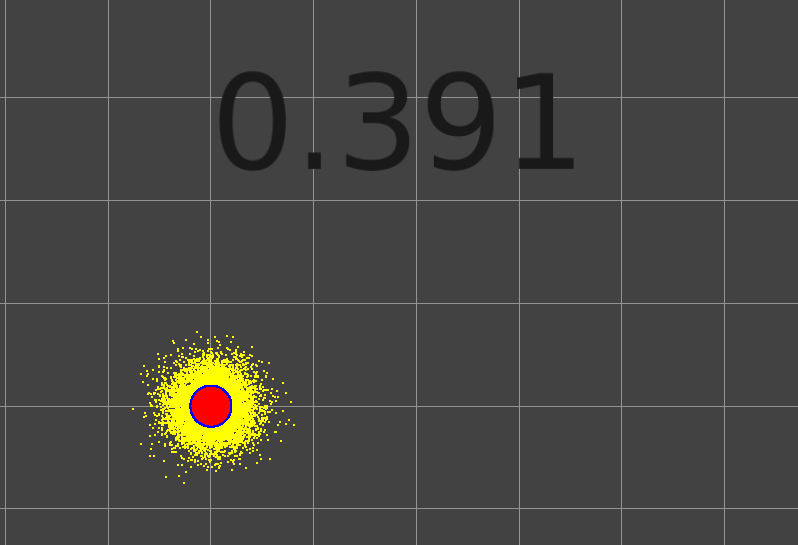
\includegraphics[width=0.8\textwidth]{figures/MultiGaussian_1_sigma.png}
\caption{Around 39\% of our sampled points fell within our ellipse for $\chi^{2} = 1$.
The contour is plotted as a red line with blue points at each sample. Red points are
samples that should fall inside the ellipse, yellow points are samples outside. The
large number indicates the percentage of the points falling inside the ellipse.}
\label{fig:multigaussian}
\end{figure}
\section{Task 3: Covariance Matrices and Covariance Projection}

\paragraph{A}

We first write $x$ and $y$ in terms of $r$ and $\theta$:

\[x = r\cos\theta\]
\[y = r\sin\theta\]


The covariance matrix in terms of $x$ and $y$ can be expressed in terms of the original covariance matrix as follows:

\[
\Sigma_{x,y} = J_{r,\theta}^{x,y}|_{r_0,\theta_0} \Sigma_{r,\theta}\left(J_{r,\theta}^{x,y}|_{r_0,\theta_0}\right)^T
\]

Where:

\[
J_{r,\theta}^{x,y} =
\left[ {\begin{array}{cc}
	\frac{\partial r}{\partial x}|_{r_0} & \frac{\partial \theta}{\partial x}|_{\theta_0}  \\[5pt]
	\frac{\partial r}{\partial x}|_{r_0} & \frac{\partial \theta}{\partial x}|_{\theta_0}  \\[5pt]
	 \end{array} } \right] =
\left[ {\begin{array}{cc}
	\cos\theta_0 & -r\sin\theta_0  \\
	\sin\theta_0 & r\cos\theta_0  \\
	 \end{array} } \right]
\]
\[
\Sigma_{r,\theta} =
\left[ {\begin{array}{cc}
	50 & 0  \\
	0 & 15 \end{array} }\right]
\]

Therefore,

\[
\Sigma_{x,y} = \left[ {\begin{array}{cc}
	\cos\theta_0 & -r_0\sin\theta_0  \\
	\sin\theta_0 & r_0\cos\theta_0  \\
	 \end{array} } \right]
	 	\left[ {\begin{array}{cc}
	50 & 0  \\
	0 & 15 \end{array} }\right]
	\left[ {\begin{array}{cc}
	\cos\theta_0 & \sin\theta_0  \\
	-r_0\sin\theta_0 & r_0\cos\theta_0  \\
	 \end{array} } \right] \]
\[
\Sigma_{x,y} = \left[ {\begin{array}{cc}
		50\cos^2\theta_0 + 0.15r_0^2\sin^2\theta_0 & 50\cos\theta_0\sin\theta_0 - 0.15r_0^2\cos\theta_0\sin\theta_0  \\[5pt]
	50\cos\theta_0\sin\theta_0 - 0.15r_0^2\cos\theta_0\sin\theta_0 & 50\sin^2\theta_0 + 0.15r_0^2\cos^2\theta_0 \\[5pt]
	 \end{array} } \right]
\]

\paragraph{B} For this sampling, we assumed that the trues values of the measurements are $\hat{r}=100$ and $\hat{\theta}=\frac{\pi}{8}$. In this way, we have a projected covariance matrix with non-zero values, which wouldn't be the case for, e.g., $\hat{r}=\hat{\theta}=0$. We also use $r_0=100$ and $\theta_0=\frac{\pi}{8}$ for the linearization.

\begin{figure}
\centering
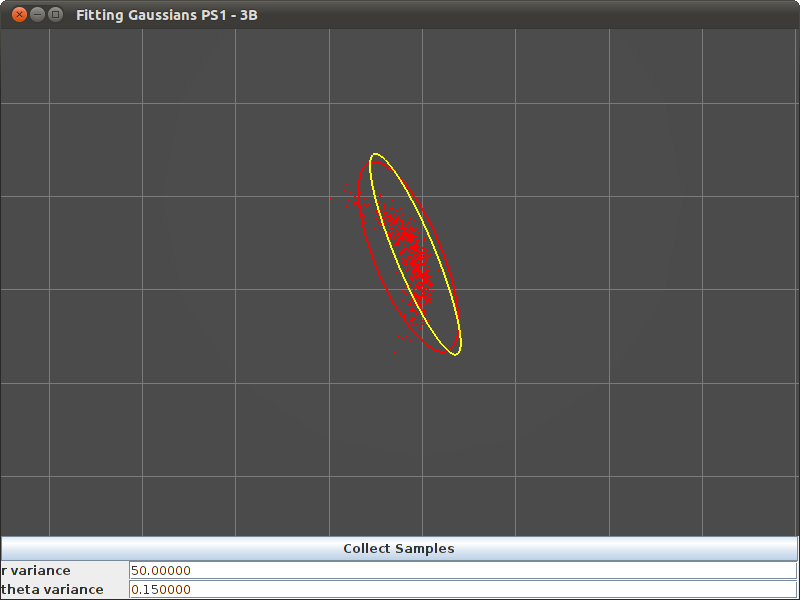
\includegraphics[width=0.8\textwidth]{figures/GaussianFit_50_0_15.png}
\caption{In red, the projection sampled points and the 3-$\sigma$ contour of the fitted multigaussian for $\sigma^2_r=50$ and $\sigma^2_\theta=0.15$ as in the assignment. In yellow, the 3-$\sigma$ contour of the projected covariance matrix.}
\label{fig:covplot_50_15}
\end{figure}

\begin{figure}
\centering
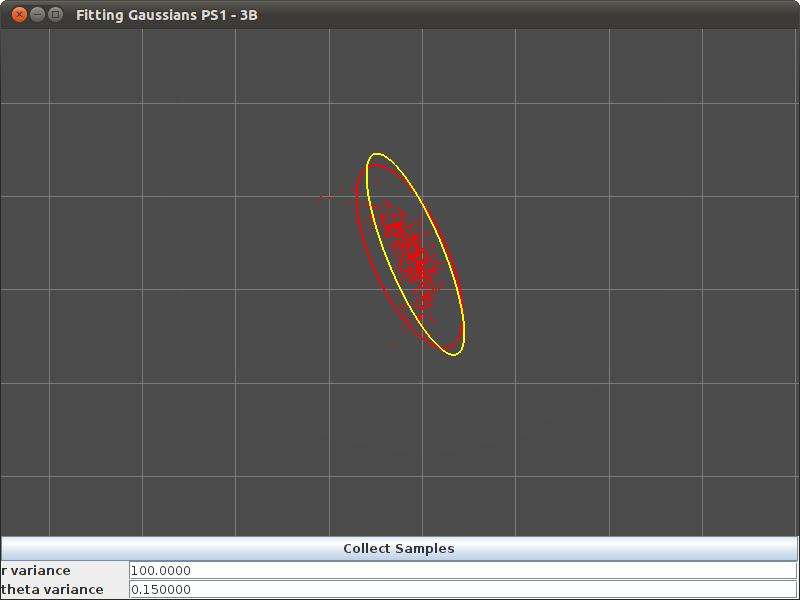
\includegraphics[width=0.8\textwidth]{figures/GaussianFit_100_0_15.png}
\caption{The points and contours for $\sigma^2_r=100$ and $\sigma^2_\theta=0.15$.}
\label{fig:covplot_100_15}
\end{figure}

\begin{figure}
\centering
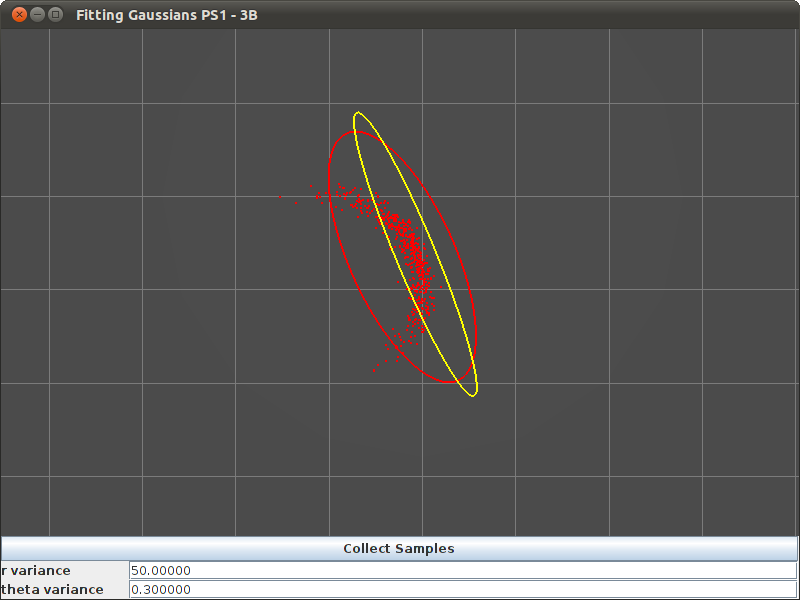
\includegraphics[width=0.8\textwidth]{figures/GaussianFit_50_0_3.png}
\caption{The points and contours for $\sigma^2_r=50$ and $\sigma^2_\theta=0.3$.}
\label{fig:covplot_50_30}
\end{figure}

\begin{figure}
\centering
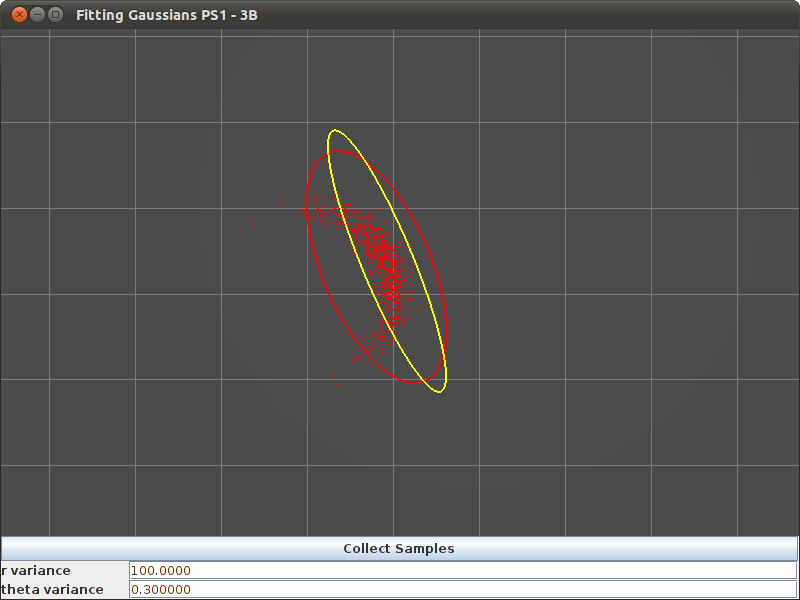
\includegraphics[width=0.8\textwidth]{figures/GaussianFit_100_0_3.png}
\caption{The points and contours for $\sigma^2_r=100$ and $\sigma^2_\theta=0.3$.}
\label{fig:covplot_100_30}
\end{figure}


% Figure~\ref{fig:covplot_50_15} is the plot for the error levels given in the assignment.
% In this case, the projected covariance matrix is a relatively good aproximation of the
% actual covariance in the data. Figure \ref{fig:covplot_100_15} is the plot when the noise
% level in $r$ increases, which makes the projected covariance even more accurate, as a
% result of the linearization). Finally, Figure \ref{fig:covplot_50_30} shows the
% consequences of increasing the error in $\theta$.

Figure~\ref{fig:covplot_50_15} shows the required plots for the error levels given
in the assignment. The 3-sigma curve for the fit points does indeed seem to contain
the majority of the samples, however, it is not a great representation of the actual distribution
of points seen. The projected 3-sigma curve is worse, still, than the fit curve as
it contains fewer of the points with high error from $w_\theta$.
Figures~\ref{fig:covplot_100_15}~and~\ref{fig:covplot_50_30} show how manipulating the
parameters influence the accuracy of the projection.

We can see from varying the noise levels that as $w_\theta$ increases, the projected
covariance matrix becomes progressively less accurate. This happens due to
linearization error. When we linearize on $\theta_0=\frac{\pi}{8}$, we are effectively
drawing a tangent at that angle of the circle defined by $\hat{r}$ and $\hat{\theta}$.
This approximation is good enough for
small errors in $\theta$, but if the noise is significant the tangent approximation
will no longer hold. Interestingly, increases in $w_r$ seem to compensate for that
effect by smudging the error caused by $w_{\theta}$ out, as can be seen in figure
\ref{fig:covplot_100_30}.

% something extra about consequences?
This has a consequence in regards to the way you choose to model your data.
Choosing the correct domain in which to model the data (in this case $(r,\theta)$ instead of
$(x,y)$) is clearly quite important. Bad linearization can be extremely damaging.
This is reminiscent of the importance of choosing a good linearization point.


\end{document}
